\setcounter{chapter}{0}
\setchapterabstract{This chapter addresses exploitative abuses and horizontal foreclosure under Article 102 TFEU. Exploitative abuses arise when a dominant firm uses market power to set excessive prices or impose unfair terms, leveraging high barriers and inelastic demand. The "excessive price" test assesses whether prices reflect product value, comparing margins and prices to benchmarks. Abusive price discrimination may distort competition or fragment markets. Horizontal foreclosure, including predatory pricing and exclusivity agreements, involves dominant firms excluding rivals in their market through aggressive pricing or loyalty rebates, analysed for anticompetitive effects, market power, and intent. Justifications like efficiency gains may be valid if they benefit consumers without notably harming competition.}
\chapter{Exploitative abuses and horizontal foreclosure}
\vspace{-1.5cm}

\setcounter{chapter}{11}
{\chaptoc\noindent\begin{minipage}[inner sep=0,outer sep=0]{0.9\linewidth}\section*{Exploitative abuses}\end{minipage}}

    A dominant firm has the power to reduce output and increase prices above the competitive level due to high barriers and inelastic demand.
    
    \begin{itemize}
        \item Charging monopoly prices would otherwise attract new entrants and/or make customers switch to lower-priced products, making the price increase unprofitable. This dynamic would in turn show that the firm is not dominant.
    \end{itemize}
    
    Monopoly prices are the reward for “winning” at the competition game, and they make firms compete aggressively, to the benefit of consumers.
    
    However, competition law imposes a limit. Article 102 prohibits unfair (excessive) prices and trading conditions, i.e., those that have “no reasonable relation to the economic value of the product supplied.”
    
    US law does not address exploitative abuses.

\section{Excessive Prices (United Brands)}

    The abuse consists in the dominant undertaking leveraging its significant market power arising from its position to reap benefits which it would not have reaped if there had been normal and sufficiently effective competition.

    \begin{itemize}
        \item “[A] price […] is excessive [when] it has no reasonable relation to the economic value of the product supplied […]. The questions […] to be determined are:
        \begin{itemize}
            \item \textbf{[Limb 1:]} whether the difference between the costs actually incurred and the price actually charged is excessive (i.e., is the profit margin excessive?),
            \item and, if the answer is in the affirmative,
            \item \textbf{[Limb 2:]} whether the price […] is either unfair in itself or when compared to competing products (comparators) (i.e., is the price excessive?).
        \end{itemize}
    \end{itemize}

    \subsection{Comparators}

        \begin{itemize}
            \item \textbf{[Limb 1 – Margin comparison]} Identify a threshold price that guarantees a satisfactory margin. If the margin goes significantly beyond that threshold, the price (margin) charged by the dominant undertaking is excessive.
            \item \textbf{[Limb 2 – Price comparison]} Determine whether the price charged is unfair in itself or when compared to competing products:
            \begin{itemize}
                \item similar products by non-dominant undertakings (comparison across competitors),
                \item the same product at different points in time (e.g., before and after dominance – comparison across time),
                \item or the same or similar products in other geographic markets (geographic comparison).
            \end{itemize}
            \item \textbf{[Sanity check 1]} If comparators are not sufficiently homogeneous, they may have to be adapted to account for specificities of the dominant firm’s product. This ensures that the “excessive” difference in price/margin is not justified by a material difference between the dominant firm’s product and the comparator.
            \item \textbf{[Sanity check 2]} The price applied by the dominant undertaking must be significantly higher than the price it would have applied if the market were competitive.
        \end{itemize}

    \subsection{Methods to identify comparators}

        \begin{itemize}
            \item “In the absence of an ubiquitous test and given the limitations inherent in all existing methods, […] to minimise the risk of errors, competition authorities should strive to examine a case by combining several methods.”
            \item “The weaknesses of one method are not necessarily remedied by applying another equally weak method. Yet, if the methods are applied independently of each other, a given limitation inherent to one of them would not affect the results obtained through the use of other methods.”
            \item “Provided that the methodologies used are, in themselves, not flawed, and that they are all applied with rigour and objectivity, the convergence of results may be taken as an indicator of the possible benchmark price in a given case.”
        \end{itemize}

    \subsubsection{Recap}

        The test to identify and sanction excessive prices is two-pronged and consists of two phases:\sn{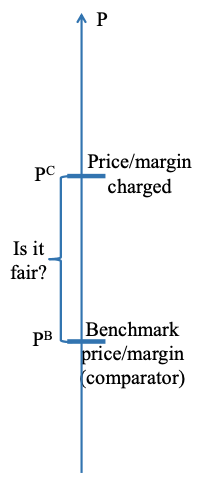
\includegraphics[width=0.5\linewidth]{recap1.png}}
        
        \begin{enumerate}
            \item Establish a fair price and a fair margin (PB) to use as a comparator/benchmark: similar products, the same product at different times or geographies, or a range.
            \item Establish whether the difference between the margin/price charged (PC) and the benchmark margin/price (PB) is fair or not.
        \end{enumerate}
        
        \begin{itemize}
            \item To be unfair, the difference must be ‘significant and persistent’.
        \end{itemize}

\section{Discriminatory prices}

    Price discrimination is not, in and of itself, an abuse. It can be beneficial in terms of allocative efficiency. If prices are marked up in inverse proportion to customers’ respective price sensitivity, it may result in increased output (it is a more efficient resource allocation if all tickets are sold, 60\% at €50 and 40\% at €10, rather than only 80\% are sold, each at €40).\sn{\Note{Preventing price discrimination may have the effect of redistributing income from poorer consumers to richer ones, depriving certain customers of access to certain products}}

        \subsubsection{Article 102(2)(c) TFEU}

            \begin{quote}
                It is an abuse for a dominant firm to apply «dissimilar conditions to equivalent transactions with other trading parties, thereby placing them at a competitive disadvantage»
            \end{quote}
            
    \subsection{Abusive price discrimination}

Price discrimination may be abusive only if it:

    \begin{itemize}
        \item Leads to the partitioning of the single European market
        \item Is exclusionary, selectively targeting competitors’ customers with low prices (if prices are below cost),
        \item Harms the competitive process by distorting competition in markets downstream/upstream, giving certain entities an unjustified economic advantage,
        \item Is exploitative, i.e., charges excessive prices to locked-in customers.
    \end{itemize}

        \subsubsection{AG Wahl (MEO, C-525/16, 20.12.2017)}

        \Example{
        \begin{itemize}
            \item “Even where an undertaking is charged higher prices than those applied to other undertakings and, as a result, suffers (or considers that it suffers) discrimination, the conduct in question will be caught by Article 102 TFEU only if it is established that it is likely to restrict competition and diminish the well-being of consumers.”
            \item Article 102 TFEU does not compel monopoly holders or dominant undertakings to apply uniform tariffs to their trading partners.
            \item “Price discrimination exercised by a dominant undertaking with regard to its trading partners may come within the scope of the prohibition of abuses of a dominant position if and only if competition between those trading partners is distorted by that discrimination.”
            \item “First, [it has to] be established that there is a competitive relationship between the trading partners of the dominant undertaking and, secondly, […] that the conduct of the dominant undertaking is actually likely to distort competition between the undertakings concerned.”
        \end{itemize}
        }

        \subsubsection{C-163/99, 29.3.2011, Portuguese Airports}

        \Example{
        \begin{itemize}
            \item ANA-EP, administrator of the Portuguese airports, applied a discriminatory system of discounts on landing charges. Discounts were “quantity discounts,” i.e., discounts offered to airlines according to the number of flights that landed at Portuguese airports. However, the system provided for high thresholds, and Portuguese airlines enjoyed the highest discounts.
            \item “where as a result of the thresholds of the various discount bands, and the levels of discount offered, discounts […] are enjoyed by only some trading parties, giving them an economic advantage which is not justified by the volume of business they bring or by any economies of scale they allow the supplier to make compared with their competitors, a system of quantity discounts leads to the application of dissimilar conditions to equivalent transactions.”
            \item In the absence of any objective justification, having a high threshold in the system which can only be met by a few particularly large partners […] or the absence of linear progression in the increase of the quantity discounts may constitute evidence of such discriminatory treatment.
            \item “The highest discount rate […] was enjoyed only by the airlines TAP and Portugalia. [T]he increase in the discount rate is appreciably greater for the highest band than for the lower bands […], which, in the absence of any specific objective justification, leads to the conclusion that the discount for the highest band is excessive in comparison with the discounts for the lower bands. […] The system in question discriminates in favour of TAP and Portugalia.”
            \item “A measure of this type […] leads to dissimilar treatment being applied to equivalent transactions, thereby affecting free competition.”
        \end{itemize}
        }

\section*{Exclusionary abuses}

        \subsubsection{Some preliminary clarifications}

            A dominant firm may strengthen its dominance by:
            \begin{itemize}
                \item Excluding or marginalizing actual rivals,
                \item Preventing the entry of potential rivals.
            \end{itemize}
            
            \begin{itemize}
                \item Excluding rivals is not necessarily anticompetitive and does not necessarily reduce consumer welfare. Consumer welfare may increase if the dominant firm competes and wins business on the merits, leading to the exit or marginalization of less efficient competitors.
                \item A dominant firm launching a new product that consumers like or using a more efficient manufacturing process that reduces its costs and prices may push less efficient rivals out of the market without reducing consumer welfare. The launch of a new product increases consumers’ choice and innovation. The development of a new process may reduce prices and increase innovation.
                \item Antitrust law forbids only abusive foreclosure (i.e., foreclosure for reasons other than competition on the merits).
            \end{itemize}

        \subsubsection{Foreclosure – horizontal and vertical}

            Foreclosure may be horizontal or vertical (or conglomerate), depending on whether foreclosure effects are on the same market in which the firm is dominant or on an upstream, downstream, or neighbouring market.

            \begin{itemize}
                \item \textbf{Horizontal foreclosure:} The dominant firm’s conduct is aimed at excluding competitors in the market in which it is dominant, through practices such as exclusive agreements, loyalty-inducing rebates, or predatory pricing.
                \item \textbf{Vertical or conglomerate foreclosure:} The dominant firm takes action to exclude firms in a downstream, upstream, or neighbouring market to the one in which it is dominant – effectively expanding its dominance to other markets. Examples include refusal to supply, margin squeeze, tying, and bundling.
                \begin{itemize}
                    \item The dominant firm is vertically integrated (upstream or downstream) or has a portfolio of products often purchased together, and
                    \item The dominant firm leverages dominance (abuse) in one market to derive benefits in another market in which it is present (but often not dominant).
                \end{itemize}
            \end{itemize}

            \Remark{Dominance, abuse and anticompetitive effects may be in different markets.}

\section{Horizontal foreclosure}

    \subsection{Predatory pricing}

        \subsubsection{The rationale underpinning predatory pricing}

            \begin{figure}[ht]
                \centering
                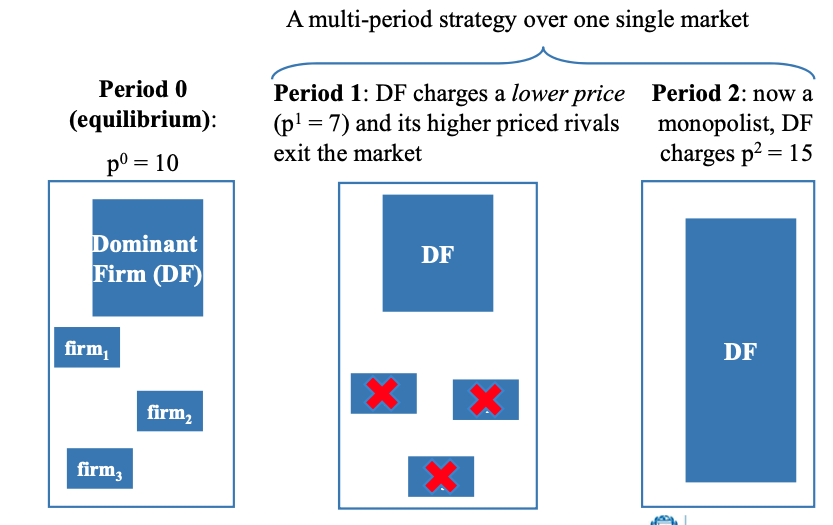
\includegraphics[width=0.75\linewidth]{image.png}
            \end{figure}

        \subsubsection{Is this strategy anticompetitive…}

            \textit{Prima facie}, yes, because:

            \begin{enumerate}
                \item \textbf{Period 1}: the dominant firm (DF) strengthens its market power by pushing rivals out of the market.
                \item \textbf{Period 2}: now a monopolist, DF raises its price to monopoly levels as there is no competitor to restrain its conduct. The reputation for acting in a predatory manner may act as a deterrent (barrier to entry) for potential competitors wishing to enter once DF increases its price.
            \end{enumerate}

            \Remark{Predation is profitable if the market is characterized by high barriers to entry (otherwise, if DF increases its price, new competitors would enter and drive the price down)}

        \subsubsection{…or not?}

            Yet, what if in period 0, the dominant firm (DF) increased its efficiency and transferred part of it to consumers by lowering its price in period 1? This equally leads to:
    
            \begin{itemize}
                \item (a) exclusion of rivals in period 1, and
                \item (b) potentially higher prices in period 2 (due to reduced competition).
            \end{itemize}
            
            The occurrence of scenarios (a) and (b) is not enough to conclude that the (exclusionary) conduct is abusive. Dominant firms have the right to compete on prices and should not be deterred from transferring efficiency gains to consumers. They should equally be able to charge the price they want (as long as it is not excessive).
            
            A further element is necessary to distinguish a legitimate price reduction from one whose only purpose or justification is to exclude rivals.

        \subsubsection{Determine who is excluded}

            To distinguish between the two mentioned scenarios, antitrust enforcers apply the as efficient competitor (AEC) test: \textit{who is excluded by the monopolist lower price?}

            \begin{enumerate}
                \item A rival who is \textbf{as efficient as} the monopolist (with less deep pockets)
                \begin{itemize}
                    \item[\(\Rightarrow\)] The market loses a good competitor
                    \item[\(\Rightarrow\)] The conduct harms the well-functioning of the competitive process
                \end{itemize}
                \item A rival who is \textbf{less efficient} than the monopolist
                \begin{itemize}
                    \item[\(\Rightarrow\)] The market loses a bad competitor
                    \item[\(\Rightarrow\)] The market is working properly
                \end{itemize}
            \end{enumerate}

        \subsubsection{How to identify as-efficient competitors?}

            Say \( P_{DF} \) is the price charged by the dominant firm. Charging \( P_{DF} \) excludes as-efficient competitors (and is thus predatory) when:

            \[
            P_{DF} < MC_{DF}
            \]
            
            (i.e., the dominant firm’s price is below its marginal cost, meaning it makes a loss on every unit it sells).
            
            To measure marginal cost (\(MC\)), antitrust enforcers use proxies. Proxies must be carefully chosen to limit the risk of over-deterrence, which would lead dominant firms not to lower their prices for fear that, by doing so, they would be found guilty of an abuse of dominance. (Type I errors deter firms from price-cutting).

        \subsubsection{Proxies for MC}

            \begin{itemize}
                \item \textbf{Total costs (TC)} are all costs sustained by the firm to produce one unit of output.\marginnote{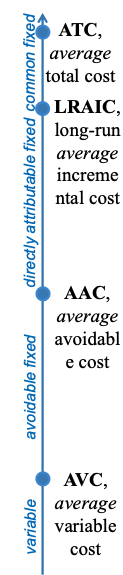
\includegraphics[width=0.5\linewidth]{image2.png}}
                \item \textbf{Long-run incremental costs (LRIC)} is the sum of the fixed and variable costs that a firm incurs when deciding to produce a particular product, referred to as ‘the increment’. LRAIC includes product-specific fixed costs (e.g., production facilities), but excludes fixed costs “common” to other products (e.g., back office functions (legal, finance), factory/warehouse covering multiple products). LRAIC may be appropriate in network industries such as telecommunications, where fixed costs are large but variable costs are low/negligible. LRAIC and ATC are good proxies for one another. In multi-product firms LRAIC is always lower than ATC, while they are the same in respect of a single product undertaking.
                \item \textbf{Avoidable costs (AC)} are the costs that a firm would avoid by ceasing a particular activity over a specified period of time (they do not include sunk costs which have already been spent and cannot be recovered); e.g., where a firm is accused of predatory pricing over an 18-month period, what costs would it have avoided if it had not produced the units that were the subject of predation? Avoidable costs include some fixed costs (those that can be avoided by not engaging in the predatory scheme), depending on the period of time in question, and variable costs, but omit any fixed costs that (would) have happened regardless. This is the standard preferred by the EC to assess ‘sacrifice’.
                \item \textbf{Variable costs (VC)} are average costs of each extra unit of output. These are costs that vary with the amount of output that a firm produces: e.g., a firm’s expenditure on items such as raw materials, energy, packaging, some labour; variable costs do not include any element of a firm’s fixed costs. Charging less than AVC is presumed abusive as every sale would generate a loss for the dominant firm.
            \end{itemize}

\newpage
        \subsubsection{The liability conditions in the EU (Akzo test)}

        The price charged by a monopolist, say \( P_{DF} \), is unlawful in two alternative scenarios:
        
        \begin{enumerate}
            \item \( P_{DF} < AVC \) (or \( AAC \)): anticompetitive intent is presumed as there is no profit-maximizing economic justification other than eliminating competitors.
            \item \( AVC < P_{DF} < ATC \) (or \( LRAIC \)) and there is exclusionary intent (i.e., pricing below ATC is part of a plan to eliminate or reduce competition).
            \begin{itemize}
                \item Direct evidence (e.g., internal documents and communications),
                \item Indirect evidence (e.g., duration and scale of losses, tactics, etc.).
            \end{itemize}
        \end{enumerate}

        \subsubsection{Defences/objective justifications}

            \begin{enumerate}
                \item Sales promotions (e.g., for the launch of a new line) may involve temporary below-cost selling.
                \item Continuous use of production facilities (even producing at a loss).
                \item For products – like skis – that are yearly renovated in shape, colours, and design for marketing (and sometimes technical) reasons, disposal of old or obsolete stock at the end of the season (better to make some return than none at all).
                \item Meeting competition. There is no absolute right for dominant firms to match non-dominant competitors’ prices if this means selling below cost. Meeting competition can be a justification only if:
                \begin{itemize}
                    \item (i) there is no anti-competitive intent,
                    \item (ii) the response is proportional to the threat to the dominant firm’s commercial interest, and
                    \item (iii) the response is reasonable considering the dominant firm’s relative market strength.
                \end{itemize}
            \end{enumerate}

        \subsubsection{Recoupment not required}

            \begin{itemize}
                \item In the US, predatory pricing can be a form of monopolization only if the alleged predator had the possibility of recouping its investment in below-cost prices. Without evidence of (potential) consumer harm, there can be no violation. Recoupment, however, may occur in a different market, which makes it difficult to measure.
                \item In the EU, the Court of Justice stated that: “proof of the possibility of recoupment of losses suffered by the application, by an undertaking in a dominant position, of prices lower than a certain level of costs [does not constitute] a necessary precondition to establishing that such a pricing policy is abusive” (France Télécom, C-202/07).
                \item The Commission is not precluded from finding that the possibility of recoupment is a relevant factor in assessing whether a pricing practice is abusive.
            \end{itemize}
        
    \subsection{Exclusivity Agreements}

        \begin{itemize}
            \item Exclusivity agreements may take the form of exclusive purchasing and exclusive supply.
            \begin{itemize}
                \item \textbf{Exclusive purchasing/single branding:} the customer must purchase certain goods or services (almost) exclusively from the dominant firm.
                \item \textbf{Exclusive supply:} the supplier can sell its products (almost) exclusively to the dominant firm.
            \end{itemize}
            \item The customer is prevented from purchasing products from, or the supplier is prevented from selling its products to, the dominant firm’s competitors.
        \end{itemize}

        \subsubsection{How exclusive}

            \begin{itemize}
                \item Exclusivity may be legal or de facto. \textbf{De facto exclusivity} consists in the commitment to purchase certain quantities amounting to a large proportion (“most of its requirements”) of the customer’s total purchases of a certain product. This may be the case, e.g., in exchange for a significant rebate (exclusivity rebate).
                \item \textbf{Stocking requirements} may in practice have the same effect as exclusive purchasing agreements. The same applies to \textbf{English clauses}, whereby the dominant firm retains the right to: 
                \begin{enumerate}
                    \item learn about its competitors’ offers, and
                    \item make an offer that matches the best alternative.
                \end{enumerate}
                \item In an Article 102 context, it is the dominant firm infringing competition rules, even though it does so by way of an agreement. The conclusion of an anti-competitive agreement can be considered an abusive unilateral act, and the only firm to be sanctioned is the dominant one.
                \item It is not a defence that the customer willingly entered into the agreement or even requested exclusivity. The issue is not the oppression of customers, but the exclusion of as-efficient competitors by foreclosing access to customers.
            \end{itemize}

        \subsubsection{Per se or not?}

            \begin{itemize}
                \item A dominant firm that “ties purchasers - even […] at their request - by an obligation or promise on their part to obtain all or most of their requirements exclusively from the said undertaking abuses its dominant position.”
                \item Despite the language, exclusivity is not a per se abuse. It is necessary to show that the conduct is capable of having anticompetitive effects: “the exclusionary effect […] may be counterbalanced, or outweighed, by advantages in terms of efficiency which also benefit the consumer. That balancing of the favourable and unfavourable effects […] can be carried out […] only after an analysis of the intrinsic capacity of that practice to foreclose competitors which are at least as efficient as the dominant undertaking.” (Intel)
                \item However, exclusivity has a high potential to produce exclusionary effects, so the burden of proof is often reversed.
            \end{itemize}

        \subsubsection{Effects}

            To determine whether the conduct may have potential anticompetitive effects, we should consider:
            
            \begin{enumerate}[label=\roman*.]
                \item the degree of market power and whether the dominant firm is an unavoidable trading partner,
                \item the share of the market affected by the conduct,
                \item the strategic importance for entry or expansion of the customers or segments targeted by the conduct,
                \item duration of the agreements and requirement of (quasi) exclusivity,
                \item intent (existence of a strategy to exclude competitors).
            \end{enumerate}
            
            Anticompetitive effects are more likely in cases of: long duration of exclusivity, strong dominant position, high percentage of the market covered by exclusivity, and an exclusionary strategy.
            
            Anticompetitive effects can be counterbalanced by pro-competitive factors:
            
            \begin{itemize}
                \item Efficiency gains (e.g., reduction of transaction costs, economies of scale, quality increase),
                \item Exclusion of free-riding (e.g., territorial exclusivity clauses),
                \item Protection when locked-in (e.g., where the supplier has to make relationship-specific investments to be able to supply that customer).
            \end{itemize}

    \subsection{Loyalty Rebates}

        \begin{itemize}
            \item With a rebate system, the purchase price depends on the customer’s behavior. Example: if the customer buys more than a certain number of pairs of skis:
                \begin{itemize}
                    \item \textbf{Incremental rebate}: each of the subsequent pair of skis costs X€ less
                    \item \textbf{Retroactive (‘all-units’) rebate}: If you buy 3, all skis purchased costs X€ less (which makes it less attractive to switch part of demand to competitors)
                \end{itemize}
            \item Most problematic rebates are so-called \textbf{exclusivity rebates}—i.e., rebates conditional on the customer obtaining all or most (>80\%) of its requirements from the dominant undertaking. To determine effects, you should consider all the circumstances surrounding the rebates, including duration and market coverage.
            \item \textbf{Conditional retroactive rebates} make customers less likely to leave the dominant firm and source a material part of their requirements from competing firms, thus making entry or expansion more difficult. Anticompetitive effects are more likely if rebates are individualized or targeted based on each customer’s size or demand, and when they cover a significant share of the market and persist for a long duration.
            \item \textbf{Foreclosure effects} are more likely if competitors cannot compete for the entire demand. That is, only part of the demand is contestable, and rivals compete only over that smaller set of customers or sales, at the effective (discounted) price.
        \end{itemize}

        \subsubsection{The liability conditions}

            Rebates are judged according to the rules on predatory pricing: is the dominant firm suffering short-run losses by offering the rebates, to obtain long-run gains from the exclusion of competitors?

            \begin{enumerate}
                \item \textbf{Firm’s position:} Determine the \textbf{contestable share}—i.e., the portion of sales that customers could switch away from the dominant firm. Part of the demand may be tied to the incumbent (e.g., replacements, spare parts).
                \item \textbf{Rebate size and retroactivity:} Estimate the \textbf{effective price}, i.e., the price that a competitor would have to offer to match the rebate over the contestable share and convince customers to switch that portion of demand to them (to compensate customers for the loss of the conditional rebate).
                \item \textbf{Apply the predatory pricing conditions} to this effective price.
                \begin{itemize}
                    \item (a) Effective price below AAC/AVC—generally capable of foreclosing as-efficient competitors (AECs) absent a convincing justification.
                    \item (b) Effective price \( > \) AAC/AVC but \( < \) LRAIC/ATC—other elements are taken into account: firm’s intent and competitors’ counterstrategies.
                    \item (c) Effective price \( > \) LRAIC/ATC—normally lawful (exception: markets where the emergence of AEC is impossible, such as natural or legal monopolies).
                \end{itemize}
            \end{enumerate}

        \subsubsection{Example of Loyalty Rebates}
            
            \begin{itemize}
                \item DomCo and MiniCo are competitors. They both offer a price of €1 per unit.
                \item DomCo has a profit margin of 19\%.
                \item CustomerCo has a requirement of 100,000 units.
                \item CustomerCo could consider buying no more than 10\% from MiniCo.
                \item DomCo asks you to advise on its proposed “go-to-market” rebate scheme.
            \end{itemize}

        \begin{figure}[ht]
            \centering
            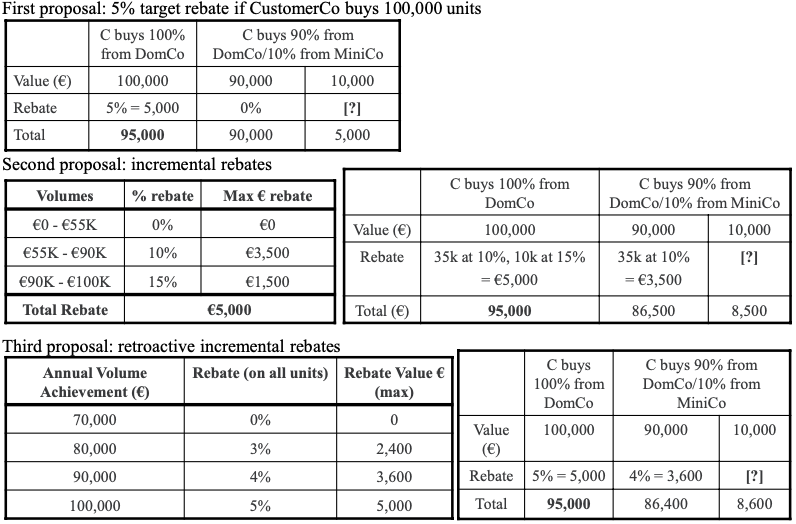
\includegraphics[width=0.75\linewidth]{image3.png}
        \end{figure}

    